\label{chap:arch}
\subsection{Hardware}

Both the main processing unit and transceiver unit of the SparrowE wireless sensor nodes are provided by an Atmel
ZigBit 900MHZ RF module. The module is composed of an ATmega 1281V 8-bit microcontroller and an
AT86RF212 RF Transceiver connected with the microcontroller via a SPI interface. The Atmega 1281V is a low power 8 bit microcontroller
which is connected to the on-board sensors of the node. In order to transmit or perform encryption operations on 
data, the microcontroller must communicate with the RF Transceiver. The Transceiver controller is also a low power chip,
capable of transmitting signals to distances of up to 6 km, as specified in the official Atmel datasheet \cite{datasheetatmel}. 
The Transceiver contains a security module compatible with AES-128. It supports hardware encryption and decryption for AES 128 ECB, but for the AES
128 CBC method only hardware encryption is supported.


\begin{figure}[ht] \centering
  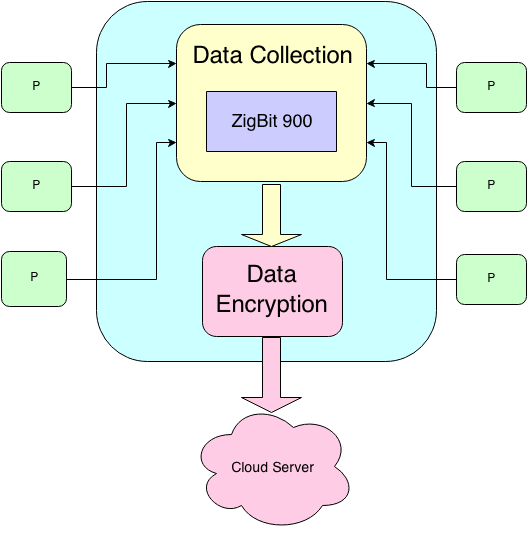
\includegraphics[width=0.5\textwidth]{img/wsn-soa-system-arch.png}
  \caption{System Architecture}
\end{figure}

\subsection{Software}

From the software perspective, the architecture is composed of three modules:
\begin{itemize}
\item data module, that
collects information from the sensors,
\item encryption module,
\item communication module.
\end{itemize}

Since the transceiver module is separated from the controller, from an efficiency perspective, it 
would be preferable to implement AES ECB and CBC algorithms as software services directly on the 
controller. Using this method, the transceiver shall be kept most of the time in an idle state, 
and the only component which will actively operate and drain the battery is the controller itself.
While the controller is one of the components with a higher power consumption rate, the implementation 
will have optimizations meant to keep the number of performed encryption operations to a minimum.
Moreover, it is important to filter data before it is packaged and sent, in order to further 
reduce the number of encryption and decryption operations which the microcontroller has to perform.

Given the available hardware resources and architecture, the proposed implementation offers 
a software solution for ensuring data security and it also uses encryption methods which can easily 
be replaced with AES ones if ported on a hardware architecture in which the transceiver is 
incorporated in the microcontroller.
